\chapter{JPEG2000}

\section{\acrshort{ISO} international standard}
\begin{itemize}
\item Developed by the \gls{JPEG} (ISO/IEC 15444\href{https://www.itu.int}{ITU}),
  the JPEG2000 standard \cite{taubman2002jpeg2000} in 2000, as a successor of
  \gls{JPEG}.
\item Mainly used in medical imaging and digital cinema.
\end{itemize}
\vspace{-2ex}
\begin{center}
  \href{https://en.wikipedia.org/wiki/Magnetic_resonance_imaging_of_the_brain#/media/File:MRI_of_Human_Brain.jpg}{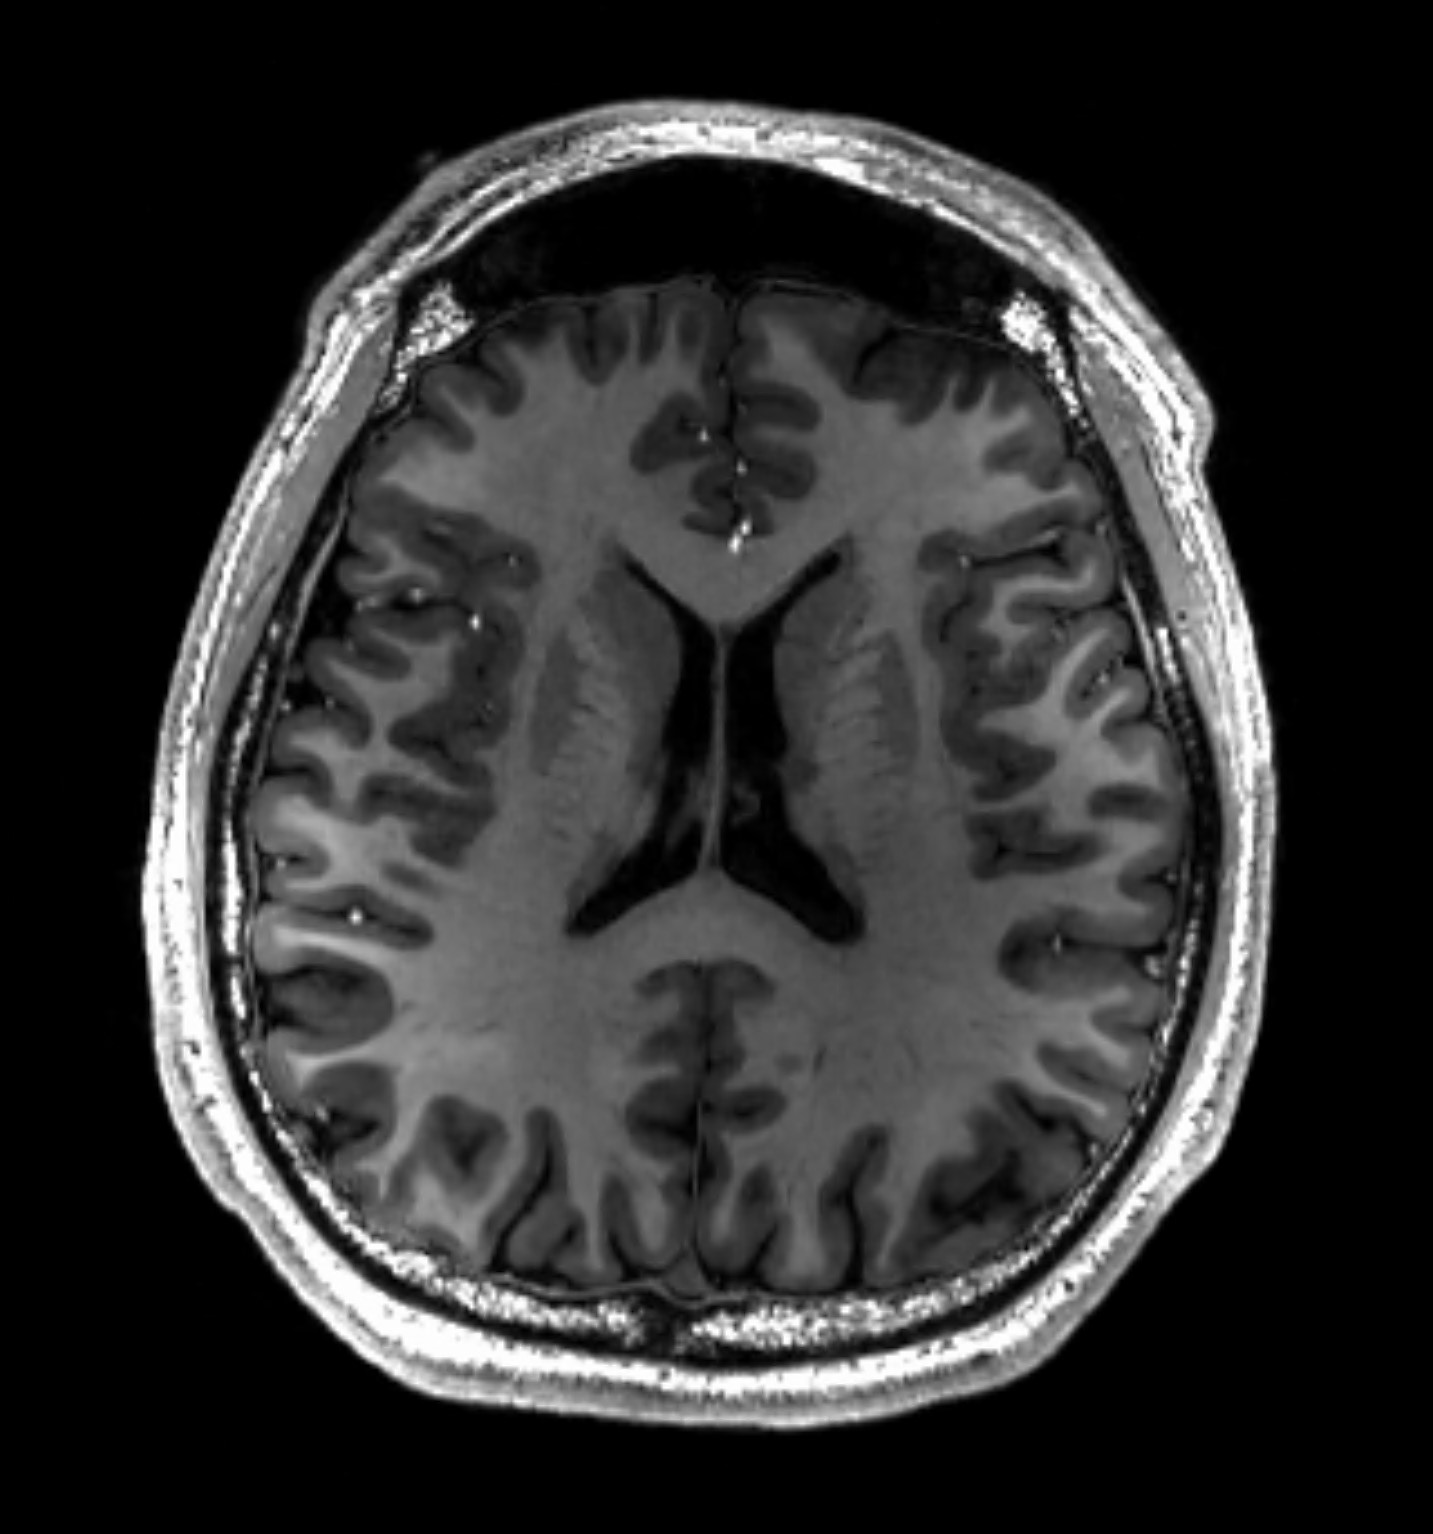
\includegraphics[width=4.0cm]{MRI_of_Human_Brain}}\\
  (click on the image)
\end{center}

\section{Lossless and lossy compression}
\begin{itemize}
\item Two different compression modes:
\item \textbf{Reversible}: Allows a perfect reconstruction of the raster image (like \gls{PNG}).
\item \textbf{Irreversible}: Unable to recover all the visual
  information, but offers a better rate/distortion performance than
  the reversible mode for the same bit-rate.
\end{itemize}

\section{16-bit per channel and several color spaces support}
\begin{itemize}
\item \popup{16 bits/pixel offers enough quality for specialized
    applications such as medicine, atronomy, etc.}{It is quite
    difficult to increase the SNR above of 16 bits because basically
    we register noise when the amplitude of signal is small.}.
\item Apart from gray-scale and \gls{RGB}, JPEG2000 supports
  \gls{YCrCb}, \gls{sRGB} \cite{sRGB_wikipedia}, \gls{CIELAB}
  \cite{CIELAB_wikipedia}, and \popup{custom}{It is posible to define
    a color transform.} \cite{houchin2001specification} color spaces.
\end{itemize}

\section{Superior compression efficiency than \gls{JPEG}}
\begin{itemize}
\item Better quality at the same bitrate compared to JPEG \cite{vruiz_J2K}.
\end{itemize}
\begin{center}
  \begin{tabular}{cc}
    \multicolumn{2}{c}{Lena at 0.1 bits/pixel} \\
    
\includegraphics[width=5cm]{lena_01} & 
\includegraphics[width=5cm]{lena_01_jp2} \\
    JPEG & JPEG2000
  \end{tabular}
\end{center}

\section{Algorithm}

\section{Lossy artifacts}

\section{Scalability}
region of interest coding

\section{Error resilience}

\section{Motion JPEG2000 (digital cinema)}

\section{Metadata}